\documentclass{article}
\usepackage[utf8]{inputenc}
\usepackage[serbian]{babel}

\usepackage[nottoc,numbib]{tocbibind}

\usepackage{hyperref}
\hypersetup{
colorlinks,
linkcolor=blue,
urlcolor=blue
}
\setlength{\topmargin}{5pt}
\usepackage{graphicx}
\graphicspath{ {./images/} }

\title{Speech emotion recognition\\
    rad iz Računarske inteligencije}
\author{Jelena Keljać 106/2018\\
        Aleksandra Pešić 15/2018}
\date{September 2022}

\begin{document}

\pagenumbering{arabic}

\maketitle
\newpage   

\renewcommand*\contentsname{Sadržaj}
\tableofcontents
\newpage

\section{Uvod}
Speech emotion recognition (SER) predstavlja problem prepoznavanja emocija na osnovu govora. Prepoznavanje emocija je nesto sto je ljudima prirodno i deo je njihove medusobne komunikacije, dok je prepoznavanje emocija od strane računara nešto što je i dalje predmet istraživanja. Prepoznavanje emocija iz govora je najkorisnije kada su u pitanju aplikacije, kada postoji neki vid komunikacije izmedu čoveka i računara. Dodavanje emocija računarima je prepoznato kao ključni faktor u tome da mašine sve više teže ljudskom ponašanju.

Dakle, cilj je da na osnovu snimaka glasova konstruišemo dobar aparat koji će što bolje klasifikovati emocije kod ljudi.

\subsection{Zvuk}
Znamo da su neke od osnovne osobina koje karakterišu ljudski glas intenzitet, visina i boja glasa.
Međutim, jedan od "problema" podataka jeste odrediti koje će karakteristike govora biti izvučene iz snimaka, na osnovu kojih će model učiti i na osnovu kojih će vršiti prepoznavanje. Zapravo, nije poznato koje će osobine uvek dovesti do najboljeg rezultata i klasifikacije. Neke informacije o tome možemo dobiti testiranjem velikog broja osobina, njihovim različitim kombinovanjem, itd. Neke od glavnih osobina zvuka su MFCC, zero-crossing rate, chroma, pitch, i druge. 

\textit{MFCC (eng. Mel-frequency cepstral coefficients)} karakteristike predstavljaju foneme (najmanje jedinice zvuka) jer se u njima manifestuje oblik vokalnog trakta (koji je odgovoran za generisanje zvuka). Predstavlja skup vrednosti, tj. koeficijenata koje sažeto opisuju oblik spektralnog sloja i često se može koristiti za opisivanje boje tona.


Mel-skala je skala odnosa percipirane frekvencije od strane ljudi sa zapravo izmerenom frekvencijom zvuka. Raznim istraživanjima su naučnici došli do zaključka da ljudi mnogo bolje primećuju razliku u frekvencijama na nizim vrednostima herz-a, te je zadatak mel-skale da skalira frekvenciju kako bi se što više približila onome što ljudski sluh može da čuje, i prevazišla te razlike.

Mel-spektrogram se izračunava primenom furijeove transformacije kako bi analizirali sadržaj frekvencije signala i kako bi ga konvertovali u mel-skalu.
MFCC se dobija prebacivanjem frekvencije iz herz-a u mel skalu, zatim primene logaritma na mel reprezentaciju zvuka, a potom primenom diskretne kosinusne tranformacije, i rezultat predstavlja spektrum mel-frekvencije u odnosu na vreme, tj kreira se mfcc.


\textit{Chroma} se odnosi na 12 različitih klasa visine tonova i predstavlja intezitet zvuka za svaku od 12 različitih klasa koje predstavljaju 12 različitih polutonova muzičke oktave. Glavno svojstvo ove odlike je ta da je otporan na promene u instrumentaciji i kvalitetu dok registruju harmonijske i melodijske karakteristike zvuka/muzike.

\textit{Zero-crossing rate} meri koliko puta u određenom vremenskom intervalu je amplituda zvučnog signala prošla kroz vrednost nula. Rezultat ove karakteristike nam može reći kad je deo zvuka glasan, tj. kad je mala stopa prolaska kroz nulu, i kad nije glasan, odnosno kad je stopa visoka, jer energija tada manja. Stoga, ovaj metod nam efikasno razdvaja zvučni i nezvučni govor.
\\
\\
\\
\section{Implementacija}
Na osnovu pronađenih podataka smo napravili dve verzije modela. Oba modela se zasnivaju na neuronskim mrežama, a detaljnije o njima ćemo kasnije u tekstu. 

\subsection{Ulazni skup podataka}
Za pravljenje našeg modela korišćena su tri seta podataka: 
    \begin{enumerate}
    \item Ryerson Audio-Visual Database of Emotional Speech and Song (Ravdess)
    \item Toronto emotional speech set (Tess)
    \end{enumerate}
\newline
Svi podaci su sačuvani u formatu .wav, tj. kao kratki glasovni snimci. Navedeni skupovi podataka su međusobno nezavisni, tj. prikupljeni iz različitih izvora. Navedeni podaci sadrze 7 različitih emocija koje model pokušava da klasifikuje i to su: sreća, tuga, bes, iznenađenje, strah, gađenje i neutralno osećanje. 

\subsection{Obrada podataka}
Zbog različitih načina čuvanja ulaznih podataka, za svaki skup smo pravili zasebnu funkciju koja će učitavati podatke iz direktorijuma i uzimati informaciju o tome koja je emocija u pitanju. Sve te funkcije smo objedinili u jednu zajedničku, load\_data. 

Za rad sa audio snimcima koristili smo biblioteku \textit{librosa} koja pruža funkcije koje omogućavaju rad sa njim. U radu smo koristili samo mfc koeficijente, jer smo primetili, na osnovu prethodnih testiranja, da se tačnost rešenja ne menja uvođenjem drugih osobina. Na objedinjenom skupu podataka smo izvlačili potrebne mfcc karakteristike iz zvuka korišćenjem \textit{librosa.feature.mfcc} funkcije. Nad novooformljenim podacima smo dalje pravili model.
Sledeći korak predstavlja podelu podataka na skup podataka za treniranje i skup podataka za testiranje, gde test skup čini 30\% od ukupnog skupa podataka. Taj skup koristimo za proveru tačnosti našeg modela. Da bi svi podaci bili ravnopravni koristimo StandardScaler koji standardizuje podatke, tj. tako transformišemo podatke da budu u normalnoj raspodeli.


\subsection{Modeli}
Oba modela su zasnovana na neuronskim mrežama. Veštačke neuronske mreže oponašaju biološke neuronske mreže. To je sistem koji se sastoji od jednog ulaznog i jednog izlaznog sloja, i skrivenog sloja, kojih može biti više kod složenijih modela. Svaki sloj se sastoji od jedinica, neurona, povezanih sa neuronima iz susednih slojeva težinskim koeficijentima.

Prvi predstavljeni model je napravljen pomoću funkcije MLPClassifier. Postavili smo batch\_size da bude malo veći, s obzirom da radimo sa većim brojem podataka.


Drugi kreirani model je napravljen pomoću keras biblioteke i modela Sequential. Postavili smo 4 sloja. Na prva 3 unutrašnja sloja smo primenili funkciju aktivacije relu. Na poslednjem sloju smo iskoristili funkciju aktivacije softmax, koja vraća vektor vrednosti između 0 i 1, koji u zbiru treba da budu 1, tj. za svaku klasu vraća verovatnoću da taj podatak pripada baš toj klasi. Model smo kompajlirali koristeći Adam funkciju za optimizaciju; metriku koju smo postavili je tačnost (eng. accuracy) i za funkciju greške koju želimo da minimizujemo smo koristili categorical\_crossentropy.


\newpage
\section {Rezultati}
Na osnovu dobijenih rezultata tačnosti i matrice konfuzije, možemo uporediti i dobiti informacije o efikasnosti naših modela.  
Prvi model je klasifikovao podatke sa tačnošću od oko 88\%. 

\begin{figure}[h]
\centering
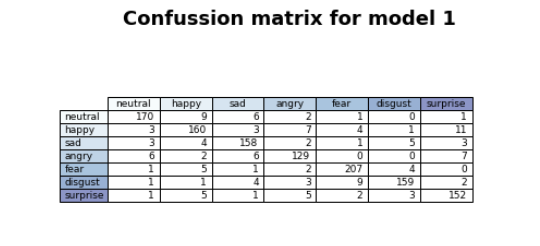
\includegraphics[scale=0.8]{matrix1.png}
\caption{Matrica konfuzije prvog modela}
\end{figure}

Na osnovu matrice konfuzije, možemo primetiti da model-1 relativno dobro klasifikuje. Najveći broj grešaka je za sreću, koje se greškom klasifikuje kao iznenađenje, a tu su i greške klasifikacije emocije gađenja kao strah.

Model-2 je za nijansu slabiji od prvog modela, sa tačnošću od oko 84\%.

\begin{figure}[ht]
\centering
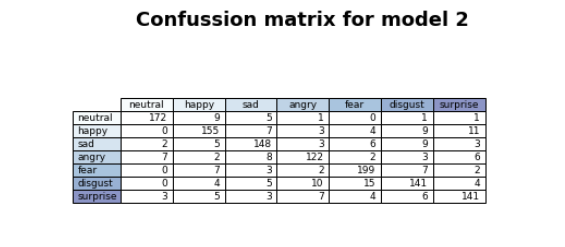
\includegraphics[scale=0.8]{matrix2.png}
\caption{Matrice konfuzije drugog modela}
\end{figure}
\newpage
Model-2 je najviše grešio za emociju gađenja, pogrešno je klasifikujući kao strah, ali i gađenje kao bes  i sreću kao iznenađenje.

\begin{figure}[h]
\centering
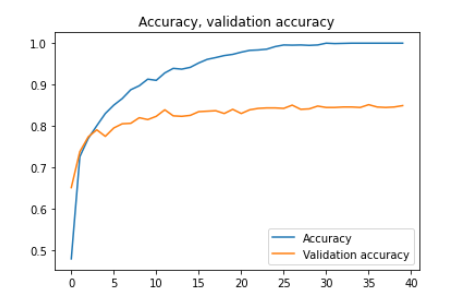
\includegraphics[scale=0.5]{val_acc.png}
\caption{Tačnost validacionog skupa}
\end{figure}

Sa grafika iznad možemo videti da je tačnost validacionog skupa oko 0,8. 
\newpage
\begin{figure}[h]
\centering
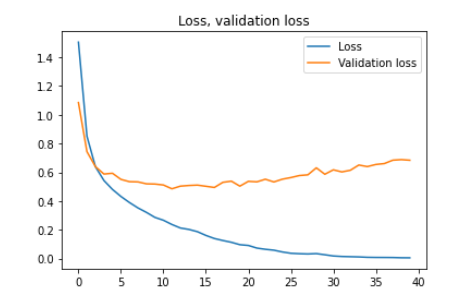
\includegraphics[scale=0.5]{val_loss.png}
\caption{Funkcija greške validacionog skupa}
\end{figure}
 
Napravljeni modeli su veoma bliski. U poređenju sa naučnim radovima i informacijama koje za sad postoje, prosečna tačnost modela za klasifikaciju emocija u glasu za slične modele kreirane pomoću MFCC je oko 73\%. 
Postoje rešenja koja se dobijaju korišćenjem drugih metoda i modela, kao i njihovim međusobnim kombinovanjem. KNN metoda ima tačnost oko 86\%; HMM (eng. Hidden Markov Model) u najboljem slučaju može imati tačnost oko 96\%, ali mu je prosečna tačnost 78\%.


\\
\newpage
\section{Zaključak}
Na osnovu dobijenih rezultata možemo videti da naše rešenje ovog problema radi dovoljno dobro, ali da ima prostora za poboljšanja.
Sa povećanjem skupa podatka ili njihovom dodatnom obradom se može povećati i tačnost modela.
Takođe, sa testiranjem i odabirom različitih parametara modela, može se dobiti model koji će raditi sa boljom tačnošću. 
Bolja rešenja se mogu dobiti i odabirom drugih vrsta modela.

\newpage

\begin{thebibliography}{6}

    \bibitem{} Babak Basharirad, Mohammadreza Moradhaseli, \textit{Speech Emotion Recognition Methods: A Literature Review}, School of Computing Asia Pacific University of Technology and Innovation (APU) Technology Park Malaysia, Bukit Jalil, Kuala Lumpur, Malaysia
    \bibitem{} Melissa Stolar, Margaret Lech, \textit{Real-Time Speech Emotion Recognition Using a Pre-trained Image Classification Network: Effects of Bandwidth Reduction and Companding}, School of Engineering, RMIT University, Melbourne, VIC, Australia 
    \bibitem{} Mohit Wadhwa,  Anurag  Gupta, Prateek Kumar Pandey, \textit{Speech emotion recognition (SER) through machine learning}, Brillio Technologies, Indian Institute of Technology, Kharagpur

    \bibitem{TESS dataset} TESS dataset:  https://www.kaggle.com/datasets/ejlok1/toronto-emotional-speech-set-tess

    \bibitem{RAVDESS dataset} RAVDESS dataset:   https://www.kaggle.com/datasets/uwrfkaggler/ravdess-emotional-speech-audio
\end{thebibliography}

\end{document}
